%%% LaTeX Template: Article/Thesis/etc. with colored headings and special fonts
%%%
%%% Source: http://www.howtotex.com/
%%% Feel free to distribute this template, but please keep to referal to http://www.howtotex.com/ here.
%%% February 2011
%%%
%%% Modified October 2015 by CDM

%%%  Preamble
\documentclass[11pt,letterpaper]{article}
\usepackage[margin=1.0in]{geometry}
\usepackage[T1]{fontenc}
\usepackage[bitstream-charter]{mathdesign}
\usepackage[latin1]{inputenc}					
\usepackage{amsmath}						
\usepackage{xcolor}
\usepackage{cite}
\usepackage{hyphenat}
\usepackage{float}
\usepackage{subfigure}
\usepackage{sectsty}
\usepackage[compact]{titlesec} 
\usepackage[tablegrid]{vhistory}
\usepackage{graphicx}
\usepackage{tabularx}
\usepackage{hyperref}
\allsectionsfont{\color{accentcolor}\scshape\selectfont}

%%% Definitions
\definecolor{accentcolor}{rgb}{0.0,0.0,0.5} 
\newcommand{\teamname}{Team C}
\newcommand{\productname}{Language Pronounciation Assisting App}
\newcommand{\coursename}{CSE 4316: Senior Design I}
\newcommand{\semester}{Summer 2017}
\newcommand{\docname}{Project Charter}
\newcommand{\department}{Department of Computer Science \& Engineering}
\newcommand{\university}{The University of Texas at Arlington}
\newcommand{\authors}{Josue C.\\ Ali S. \\ Norween J. \\ Xiwen D. \\ Kristen R.}
\hypersetup{
    colorlinks=true,
    urlcolor=blue,
}

\setcounter{secnumdepth}{4}

\titleformat{\paragraph}
{\normalfont\normalsize\bfseries}{\theparagraph}{1em}{}
\titlespacing*{\paragraph}
{0pt}{3.25ex plus 1ex minus .2ex}{1.5ex plus .2ex}

%%% Headers and footers
\usepackage{fancyhdr}
	\pagestyle{fancy}						% Enabling the custom headers/footers
\usepackage{lastpage}	
	% Header (empty)
	\lhead{}
	\chead{}
	\rhead{}
	% Footer
	\lfoot{\footnotesize \teamname \ - \semester}
	\cfoot{}
	\rfoot{\footnotesize page \thepage\ of \pageref{LastPage}}	% "Page 1 of 2"
	\renewcommand{\headrulewidth}{0.0pt}
	\renewcommand{\footrulewidth}{0.4pt}

%%% Change the abstract environment
\usepackage[runin]{abstract}			% runin option for a run-in title
%\setlength\absleftindent{30pt}			% left margin
%\setlength\absrightindent{30pt}		% right margin
\abslabeldelim{\quad}	
\setlength{\abstitleskip}{-10pt}
\renewcommand{\abstractname}{}
\renewcommand{\abstracttextfont}{\color{accentcolor} \small \slshape}	% slanted text

%%% Start of the document
\begin{document}

%%% Cover sheet
{\centering \huge \color{accentcolor} \sc \textbf{\department \\ \university} \par}
\vspace{1 in}
{\centering \huge \color{accentcolor} \sc \textbf{\docname \\ \coursename \\ \semester} \par}
\vspace{0.5 in}
\begin{figure}[h!]
	\centering
   	
\includegraphics[width=0.40\textwidth]{figures/logo12.png}
\end{figure}
\vspace{0.5 in}
{\centering \huge \color{accentcolor} \sc \textbf{\teamname \\ \productname} \par}
\vspace{0.5 in}
{\centering \large \sc \textbf{\authors} \par}
\newpage


%\vspace{1 in}
%\centerline{January 13th, 2012}
%\newpage

%%% Revision History
\begin{versionhistory}
  	\vhEntry{0.1}{07.03.2017}{}{document creation}
  	\vhEntry{0.2}{12.13.2017}{}{closeout materials}
\end{versionhistory}
\newpage

%%% Table of contents
\tableofcontents
\newpage

%%% List of figures and tables (optional)
\listoffigures
%\listoftables
\newpage

%%% Agile project charter sections
\section{Vision}
Our project vision is to improve current pronounciation-training technology, by providing real-time feedback on word accuracy.

\section{Mission}
Our mission is to assist people with improving their foreign language pronounciation skills.

\section{Success Criteria}
A successful scenario for us is one where we've developed a mobile application which gives feedback to the user for their distance to a regular speaker's pronounciation of the same word.


%%% Remaining project charter sections
\section{Background}
Our team has little to no experience in designing mobile applications, and we are required to design a language recognition application that studied the Python libraries of neural networks to instantiate the correct pronunciations of words, the requirement that is stated by the sponsors that the computing logic of the application needs to be computing in the cloud either using Microsoft Azure, Amazon WPS, or Google Cloud, which then will tie into an Android application guided user interface
designed using Android Studio and Java and only display the results of the logic.

\section{Related Work}
Currently there are many Speech and Text Recognition software out in the market, both on iOS and Android platforms, however none of the software achieve what we are trying to achieve. However, we can look at these applications to provide us with a starting point in the initial design of our mobile app. We are trying to appropriate a dictation software that can recognize speech and return the proper pronunciation of the verbiage being used.

\section{System Overview}
In order to minimize the burden of processing on the individual clients that utilize our system the application takes a lightweight-client approach to the traditional client-server application.

\begin{figure}[h!]
	\centering
 	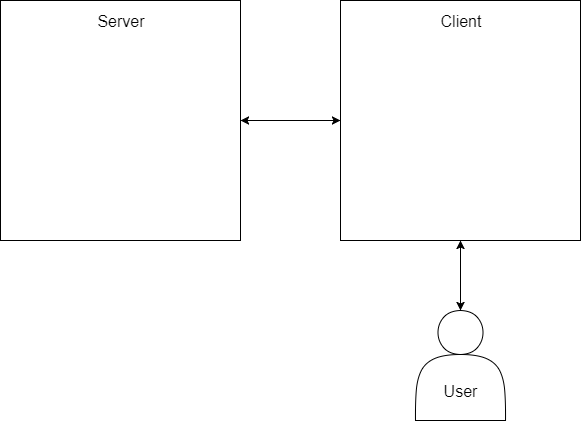
\includegraphics[width=0.60\textwidth]{images/layers}
 \caption{A high-level data-flow diagram for our application}
\end{figure}

\subsection{Client Layer}
The client will function as the HMI between our system and the user. It consists of a UI, and methods by which it may communicate with the server.

\subsection{Server Layer}
The server will function as the work-horse for the application. It's purpose is to host the visualization function which will map an input of word, audio to a distance metric in the form of x, y co-ordinates.

\section{Roles \& Responsibilities}
The product owner of our project is Nowreen Jilaney. She will be in charge of making sure that the team knows all of the specifications for the product and will be the lead in interacting with the sponsors.
The Scrum Master is Syed Ali.
He will be in charge of making sure the team members know what they are working on and keeping the team on track.

\section{Facilities \& Equipment}
As our product is a mobile app, there is no specialized equipment that we need.
We will need licenses for the environments we will be using to code the app, such as the environment for Python.
We will also need access to a cloud server for computing and storage.

\section{Cost Proposal}
Details for the preliminary budget, as well as the current \& pending support are below.

\subsection{Preliminary Budget}
The preliminary budget for our project is \$800.

\subsection{Current \& Pending Support}
We have not currently spent any of our budget.
Our pending spending will include monthly costs for access to the cloud computing service from Amazon Web Service, AWS.

\section{Documentation \& Reporting}
In this section, you will describe all of the various artifacts that you will generate and maintain during the project lifecycle. Describe the purpose of each item below, how the content will be generated, where it will be stored, how often it will be updated, etc. 

\subsection{Project Charter}
Details for the project charter are contained within this document.

\subsection{Product Backlog}
\begin{table}[htbp]
    \centering
    \begin{tabularx}{\textwidth}{l}
        Task\\
        \hline
        Investigate Neural Network Python Packages\\
        Create Bare-bones Android Application\\
        Implement server-side code on AWS\\
    \end{tabularx}
\end{table}

\subsection{Sprint Planning}
\begin{table}[htbp]
    \centering
    \begin{tabularx}{\textwidth}{l|l}
        Backlog Item & Est. Time\\
        \hline
        Research on basic human speech features & 12\\
        Research on neural networks & 12\\
        Research on Fourier transform and Formant frequencies & 4\\
        Record samples of common US English (enUS) words & 2\\
        Build an API on a mobile platform to send the input to the server, properly display output & 14\\
        Build a prototype in Android studio & 12\\
        Research on various Python libraries & 2\\
        Implement Fourier transform, Formant frequency, and spectrogram in Python. & 10\\
        Use a speech signal (word) as a sample & 10\\
        Gather information on cloud development & 4\\
    \end{tabularx}
\end{table}

\subsubsection{Sprint Goal}
\begin{itemize}
    \item  Develop an understanding of basic human speech, neural networks, Fourier transform, and Formant frequencies.
    \item  Gather all data and supplies required for Android application development.
\end{itemize}

\subsubsection{Sprint Backlog}
\begin{table}[htbp]
    \centering
    \begin{tabularx}{\textwidth}{l|l|l|l|l|l|l}
        User Story & Tasks &    Mon & Tue & Wed & Thur & Fri\\
        \hline
        & Research on basic human speech features & 3 & 3 & 3 & 3 & 0\\
        & Research on neural networks & 3 & 3 & 3 & 3 & 0\\
        & Research on Fourier transforms and Format frequencies & 2 & 2 & 0 & 0 & 0\\
        & Record samples of common US English (enUS) words & 1 & 1 & 0 & 0 & 0\\
        1 & Learn Javascript and HTML & 1 & 1 & 1 & 1 & 1\\
        1 & Create a webpage using JavaScript and HTML & 1 & 1 & 1 & 1 & 1\\
        1 & Design Web Interface & 1 & 1 & 1 & 1 & 1\\
        1 & Test the program & 1 & 1 & 1 & 1 & 1\\
        2 & Download proper Android development software & 1 & 0 & 0 & 0 & 0\\
        2 & Implement recording option for the user & 1 & 1 & 1 & 1 & 1\\
        2 & Store recorded word & 2 & 0 & 0 & 0 & 0\\
        2 & Display the word on the screen as a plot & 2 & 2 & 0 & 0 & 0\\
        & Research on various python libraries & 2 & 0 & 0 & 0 & 0\\
        & Implement Fourier transform, Formant frequency, and spectrogram in Python. Use a speech signal (word) as a sample & 4 & 4 & 4 & 4 & 4\\
    \end{tabularx}
\end{table}
\begin{table}[htbp]
    \centering
    \begin{tabularx}{\textwidth}{l|l}
        User Story No. & Description\\
        \hline
        1 & Build an API on mobile platform\\
        1 & Build a prototype in Android Studio\\
    \end{tabularx}
\end{table}

\subsubsection{Task Breakdown}
Lorem ipsum dolor sit amet, quidam omnesque ea vis. Eum an aliquip legendos recusabo. Mea ex purto natum, ne movet fuisset sit. Labore audiam eos ad, facer ornatus posidonium ne ius, et eos duis delenit nusquam.

\subsection{Sprint Burndown Charts}
Lorem ipsum dolor sit amet, quidam omnesque ea vis. Eum an aliquip legendos recusabo. Mea ex purto natum, ne movet fuisset sit. Labore audiam eos ad, facer ornatus posidonium ne ius, et eos duis delenit nusquam.

\begin{figure}[h!]
    \centering
    
\includegraphics[width=0.5\textwidth]{figures/test_image}
    \caption{Example sprint burndown chart}
\end{figure}

\subsection{Sprint Retrospective}
Lorem ipsum dolor sit amet, quidam omnesque ea vis. Eum an aliquip legendos recusabo. Mea ex purto natum, ne movet fuisset sit. Labore audiam eos ad, facer ornatus posidonium ne ius, et eos duis delenit nusquam.

\subsection{Individual Status Reports}
Lorem ipsum dolor sit amet, quidam omnesque ea vis. Eum an aliquip legendos recusabo. Mea ex purto natum, ne movet fuisset sit. Labore audiam eos ad, facer ornatus posidonium ne ius, et eos duis delenit nusquam.

\subsection{Engineering Notebooks}
Lorem ipsum dolor sit amet, quidam omnesque ea vis. Eum an aliquip legendos recusabo. Mea ex purto natum, ne movet fuisset sit. Labore audiam eos ad, facer ornatus posidonium ne ius, et eos duis delenit nusquam.

\subsection{Closeout Materials}
Lorem ipsum dolor sit amet, quidam omnesque ea vis. Eum an aliquip legendos recusabo. Mea ex purto natum, ne movet fuisset sit. Labore audiam eos ad, facer ornatus posidonium ne ius, et eos duis delenit nusquam.

\subsubsection{System Prototype}
Lorem ipsum dolor sit amet, quidam omnesque ea vis. Eum an aliquip legendos recusabo. Mea ex purto natum, ne movet fuisset sit. Labore audiam eos ad, facer ornatus posidonium ne ius, et eos duis delenit nusquam.

\subsubsection{Project Poster}
Lorem ipsum dolor sit amet, quidam omnesque ea vis. Eum an aliquip legendos recusabo. Mea ex purto natum, ne movet fuisset sit. Labore audiam eos ad, facer ornatus posidonium ne ius, et eos duis delenit nusquam.

\subsubsection{Web Page}
Lorem ipsum dolor sit amet, quidam omnesque ea vis. Eum an aliquip legendos recusabo. Mea ex purto natum, ne movet fuisset sit. Labore audiam eos ad, facer ornatus posidonium ne ius, et eos duis delenit nusquam.

\subsubsection{Demo Video}
Lorem ipsum dolor sit amet, quidam omnesque ea vis. Eum an aliquip legendos recusabo. Mea ex purto natum, ne movet fuisset sit. Labore audiam eos ad, facer ornatus posidonium ne ius, et eos duis delenit nusquam.

\subsubsection{Source Code}
Lorem ipsum dolor sit amet, quidam omnesque ea vis. Eum an aliquip legendos recusabo. Mea ex purto natum, ne movet fuisset sit. Labore audiam eos ad, facer ornatus posidonium ne ius, et eos duis delenit nusquam.

\subsubsection{Source Code Documentation}
Lorem ipsum dolor sit amet, quidam omnesque ea vis. Eum an aliquip legendos recusabo. Mea ex purto natum, ne movet fuisset sit. Labore audiam eos ad, facer ornatus posidonium ne ius, et eos duis delenit nusquam.

\subsubsection{Hardware Schematics}
Lorem ipsum dolor sit amet, quidam omnesque ea vis. Eum an aliquip legendos recusabo. Mea ex purto natum, ne movet fuisset sit. Labore audiam eos ad, facer ornatus posidonium ne ius, et eos duis delenit nusquam.

\subsubsection{CAD files}
Lorem ipsum dolor sit amet, quidam omnesque ea vis. Eum an aliquip legendos recusabo. Mea ex purto natum, ne movet fuisset sit. Labore audiam eos ad, facer ornatus posidonium ne ius, et eos duis delenit nusquam.

\subsubsection{Installation Scripts}
Lorem ipsum dolor sit amet, quidam omnesque ea vis. Eum an aliquip legendos recusabo. Mea ex purto natum, ne movet fuisset sit. Labore audiam eos ad, facer ornatus posidonium ne ius, et eos duis delenit nusquam.

\subsubsection{User Manual}
Lorem ipsum dolor sit amet, quidam omnesque ea vis. Eum an aliquip legendos recusabo. Mea ex purto natum, ne movet fuisset sit. Labore audiam eos ad, facer ornatus posidonium ne ius, et eos duis delenit nusquam.

\newpage

%%% References
\bibliographystyle{plain}
\bibliographystyle{reference/IEEEtran_custom}
\bibliography{reference/refs}{}

\end{document}
